\section{Judas}
\label{met:Judas}

\subsection{Overview}

Judas, formerly known as Emerald \cite{projthesis}, is a Julia package we've created for internal use for members at \acrshort{cgf}. Our work started last fall, when we saw a limitation of current applications at \acrshort{cgf} for loading \acrshort{das} data from local servers into programs to be able to process and further analyze these data. We chose to write this package in Julia both due to its high performance, and members' familiarity with similar languages such as MatLab and Python. With Julia, we could draw strengths from its ecosystem and build systems to create an easy-to-use library for members to familiarize themselves with. We did so by starting off with a simple python program, that read multiple \acrshort{hdf5} files storing \acrshort{das} data into dataframes. From here, we parallellized certain parts of the code, and opted to store processed data in memory mapped files instead of loading large matrices into memory. This allowed us to work with more data at the same time, as well as decreasing the overall wall time and memory consumption.  

In this section, we will be looking at what changes has been made ever since, from improvements of existent code, to new methods added and the availability of the library for members at \acrshort{cgf}. \\

Judas is designed in a data oriented manner, without object oriented features. We split our program in 4 parts: loading \acrshort{das} data from \acrshort{hdf5} files, signal processing, matrix operations and utilities for plotting. A full overview over our package design can be seen in \ref{fig:judasoverview}.\\

\begin{figure}[!h]
    \centering
    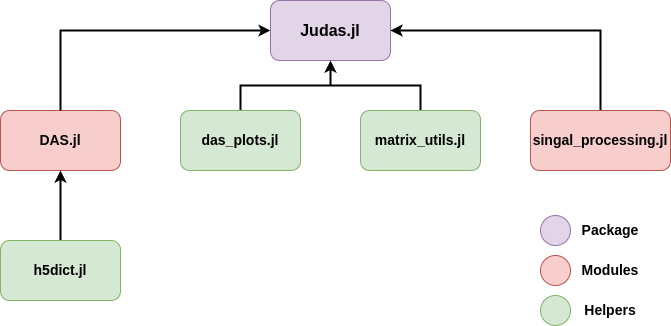
\includegraphics[scale=.6]{figures/judas_overview.png}
    \caption{Overview over our package \texttt{Judas}}
    \label{fig:judasoverview}
\end{figure}

In comparison to Emerald, Judas now contains methods for signal processing and general utilities for plotting and loading files. File I/O is also improved by reducing overall memory usage, and better parallelization techniques.
\ref{fig:apiflow} shows which core functions have been changed or added to our program. Aside from these, all other utility functions are completely new. \\

\begin{figure}[!h]
    \centering
    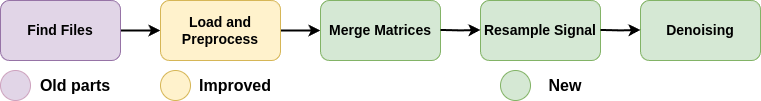
\includegraphics[scale=0.5]{figures/dataflow.png}
    \caption{Dataflow from we read HDF5 files to we are ready to train}
    \label{fig:apiflow}
\end{figure}


\subsection{Preprocessing functions}

\subsubsection{Channel Decimation}

The stored \acrshort{das} data does not store every single channel as mentioned. The \acrfull{roi} gives us information about which channels are included. To improve on our current code, we allow for channel selection through a \texttt{step} parameter. In table \ref{tab:experiment_data}, we see that every 4th sensor is stored. From this, we allow the \texttt{step} parameter to select the effective distance between each channel. Thus, we can effectively choose on which scale the \acrshort{das} data is to be analyzed. If the previous channel distance was about \qty{4}{\meter}, by assigning \texttt{step} to 25, every \qty{100}{\meter} would be loaded. \\

\subsubsection{Loading \acrshort{das} data}

The \texttt{DAS.jl} file has undergone massive changes. The primary modifications revolves around the \texttt{DASDataFrame} structure, and improvements in parallelization as well as memory consumption. Previously, we wrote matrix data to a single a binary file. Now, this data is distributed across multiple files, which can be loaded into memory as needed. This new method optimizes data retrieval and storage efficiency. Furthermore, we handle some potential race conditions to the parallelized section by synchronizing every process after they're done with local work. 

\lstinputlisting[label={code:parproc},caption=Parallel processing of \acrshort{das} signal matrices, language=Julia]{code/load_das_files.jl}

In code listing \ref{code:parproc}, we see how the function \texttt{process\_DAS\_chunk} is changed. By synchronizing the entire for-loop, we avoid problems of \acrshort{das} files not being processed before further loading them. Instead of directly writing to a binary file, we memory map the processed data, before we synchronize the processed matrix with the file loaded in memory.

The return type of the \texttt{load\_DAS\_files} function has also been slightly modified. In the previous implementation, a \texttt{DASDataFrame}, a vector of timestamps was stored for each sample, which proved to be redundant. The revised approach leverages the inherent regularity of the sampling process. By storing only the initial timestamp and the sampling rate $T$, subsequent timestamps can be efficiently calculated using the formula:

$$timestamp = start\_time + MilliSecond(idx \times T \times 1000)$$

This in-place calculation can be vectorized and broadcasted, resulting in improved computational efficiency. This modification not only reduces memory usage but also maintains all essential temporal information required for subsequent data processing. Additionally, we store the number of rows in a single file, the amount of files processed, and the \texttt{step} parameter we defined earlier, to get an accurate channel distance after channel decimation.\\

\begin{figure}[!h]
\centering
\begin{subfigure}{.45\textwidth}
  \centering
  \lstinputlisting[language=Julia]{code/dasstructold.jl}
  \caption{Old \texttt{DASDataFrame} struct}
  \label{fig:olddasstc}
\end{subfigure}%
\hfill
\begin{subfigure}{.45\textwidth}
  \centering
  \lstinputlisting[language=Julia]{code/dasstruct.jl}
  \caption{New \texttt{DASDataFrame} struct}
  \label{fig:newdasstc}
\end{subfigure}
\caption{Comparison between different versions of the DAS struct}
\label{fig:dasstccmp}
\end{figure}


\subsubsection{Parallel Resampling}

One of the ways we're able to reduce memory consumption of our program is to resample the signal matrix. What we want to do, is to resample by each sensor, and then combining the results into a new resampled matrix. As we've seen, the original frequency is $2000Hz$, but we want to resample down to $100Hz$, thus only storing $5\%$ of the original data. The following code below shows the implementation of our \texttt{parallel\_resample} function. \\

\lstinputlisting[label={code:parres}, caption=Implementation of parallel resampling, language=Julia]{code/parallel_resample.jl}

Our parallel resampling approach optimizes performance through memory management and parallel processing techniques. The algorithm proceeds as follows:

\begin{enumerate}
    \item \textbf{Memory Preallocation}: We begin by preallocating a \texttt{SharedMatrix}. This matrix can be accessed and modified by all processes, avoiding manual communication between processes. This is crucial for performance, as it also avoids dynamic memory allocations during the resampling process.
    \item \textbf{Parallel Processing}: We utilize the \texttt{pmap} function from the \texttt{Distributed.jl} package to distribute the resampling workload across multiple processes. Each process is assigned a subset of columns from the input data, allowing for parallel resampling of multiple channels.
    \item \textbf{Resampling}: Within each process, we apply the \texttt{resample} function (from \texttt{DSP.jl}) to individual columns, resampling each channel independently.
    \item \textbf{Data Collection}: To gather the results from the processes, we employ an optimized loop structure. The \texttt{@inbounds} macro disables bounds checking, eliminating the overhead of boundary checks during array checks. The \texttt{@simd} macro is applied to hint to the compiler to allow for loop reordering, potentially enabling vectorization.
\end{enumerate}



\subsubsection{Denoising \acrshort{das} signals}

\lstinputlisting[caption=Denoise function, language=Julia]{code/denoise.jl}

The last addition to \texttt{Judas.jl} is the \texttt{denoise} function. It combines tapering and digital filtering techniques, resulting in an efficient algorithm for \acrshort{das} signal denoising. The function proceeds as follows:

\begin{enumerate}
    \item \textbf{Input validation}: \texttt{denoise} is only performed if tapering is enabled and we are certain the input data is a matrix.
    \item \textbf{Tapering}: A Tukey window (tapered cosine) is applied to mitigate edge effects. Subsequentually, we broadcast the taper across all channels simultaneously.
    \item \textbf{Cutoff Frequency Normalization}: Following, we   normalize the cutoff frequecies by the Nyquist frequency \cite{schmogrow2012nyquist}.
    \item \textbf{Digital Filtering}: We utilize the  \texttt{filtfilt} function to apply a zero-phase digital filter, which preserves the phase of the original signal. The filter type provided can be either a lowpass, highpass or a bandpass filter, allowing for selecting approriate filtertype for the scenario. The Butterworth filter design offers a maximally flat frequency response in the passband, providing optimal reduction of noise.
\end{enumerate}

\subsection{General Usage and Distribution}

Our main goal with \texttt{Judas.jl} iss to provide a high performance and easy-to-use library for members at \acrshort{cgf}. To illustrate the ease of use, the following code listing \ref{code:judas} showcases its simplicity and how users easily can use it alongside other packages. \\

\lstinputlisting[label={code:judas}, caption=run.jl, language=Julia]{code/judas_usage.jl}

To run this code, we can either add processes within the program with the \texttt{addprocs(amount::Int)} function, or by starting Julia in a distributed environment as shown below.

\begin{lstlisting}[style=shellcommand, language=bash, caption=How to run a simple script containing Judas snippets]
(*@\textcolor{promptcolor}{\$}@*) julia -p 4 run.jl
\end{lstlisting}

In addition to the methods we've described in detail, there exist multiple helper methods for plotting and reading/writing \acrshort{das} data. \texttt{Judas.jl} v1.1.0 is currently available for use for members at \acrshort{cgf}. 

